%!TEX root = thesis.tex

\chapter{Appendix}
\label{chap:app}

\section{Testing the updated NWB motorways}
\label{sec:nwb_updated}

In an effort to resolve some of the problems regarding \ac{nwb}'s georeferencing issues, \ac{ndw} commissioned several commercial projects. One of these projects performed a \ac{bgt}-based refinement of municipal road (\ac{g_road}) centrelines, and these improvements already form part of the regular \ac{nwb} release. A more recent project performed a similar refinement of motorway (\ac{r_road}) centrelines. Like the commercial counterpart of the present research, this project also relied entirely on \ac{dtb}. I was given access to preliminary results of these updated geometries, and present the results of testing them in this additional section.

\subsection{Updated NWB geometry}
\label{sub:nwb_updated_geometry}

My project was affected noticeably by the coarse georeferencing of \ac{nwb}. While it is theoretically possible to derive elevations for the road network that comply with the 20 cm elevation accuracy requirement, the elevations will not necessarily reflect elevation at the desired 2D locations where \ac{nwb}'s georeferencing is particularly inaccurate. Furthermore, the fact that it is impossible to predict where the centreline lies on a given road surface (and in some places, \textit{whether} it even lies on it) caused practical issues with my algorithms.

Figure \ref{fig:nwb_updated_geometry} shows the differences between some original \ac{nwb} geometries and the updated ones in the \textit{Knooppunt Deil} area. The displacements are typically on the 0-1 m scale, but I observed up to 5 m deviations in certain locations, as also suggested by the nominal accuracy of the dataset. In the region shown by the figure, the displacement is 1-2.5 m in the locations labelled as "large shifts in NWB's location". As noted in various places in this report, problems are most common in sharp bends. Accordingly, the updated geometry shows the largest displacement relative to the original in such places. The second most common location is where no \ac{nwb} vertices are present for hundreds of metres due to the local straightness of certain motorways. This type of simplification results in several metres of displacement that may be present for most of the simplified length of the given road.

As the centrelines were "re-centred" using \ac{dtb} lines, the refinements were only carried out for motorways, and only where sufficient \ac{dtb} data is present, i.e. at least the two road edge lines. In the testing dataset shown by Figure \ref{fig:nwb_updated_geometry}, this means about 75\% of the total length of the roads.

\begin{figure}[h]
    \centering
    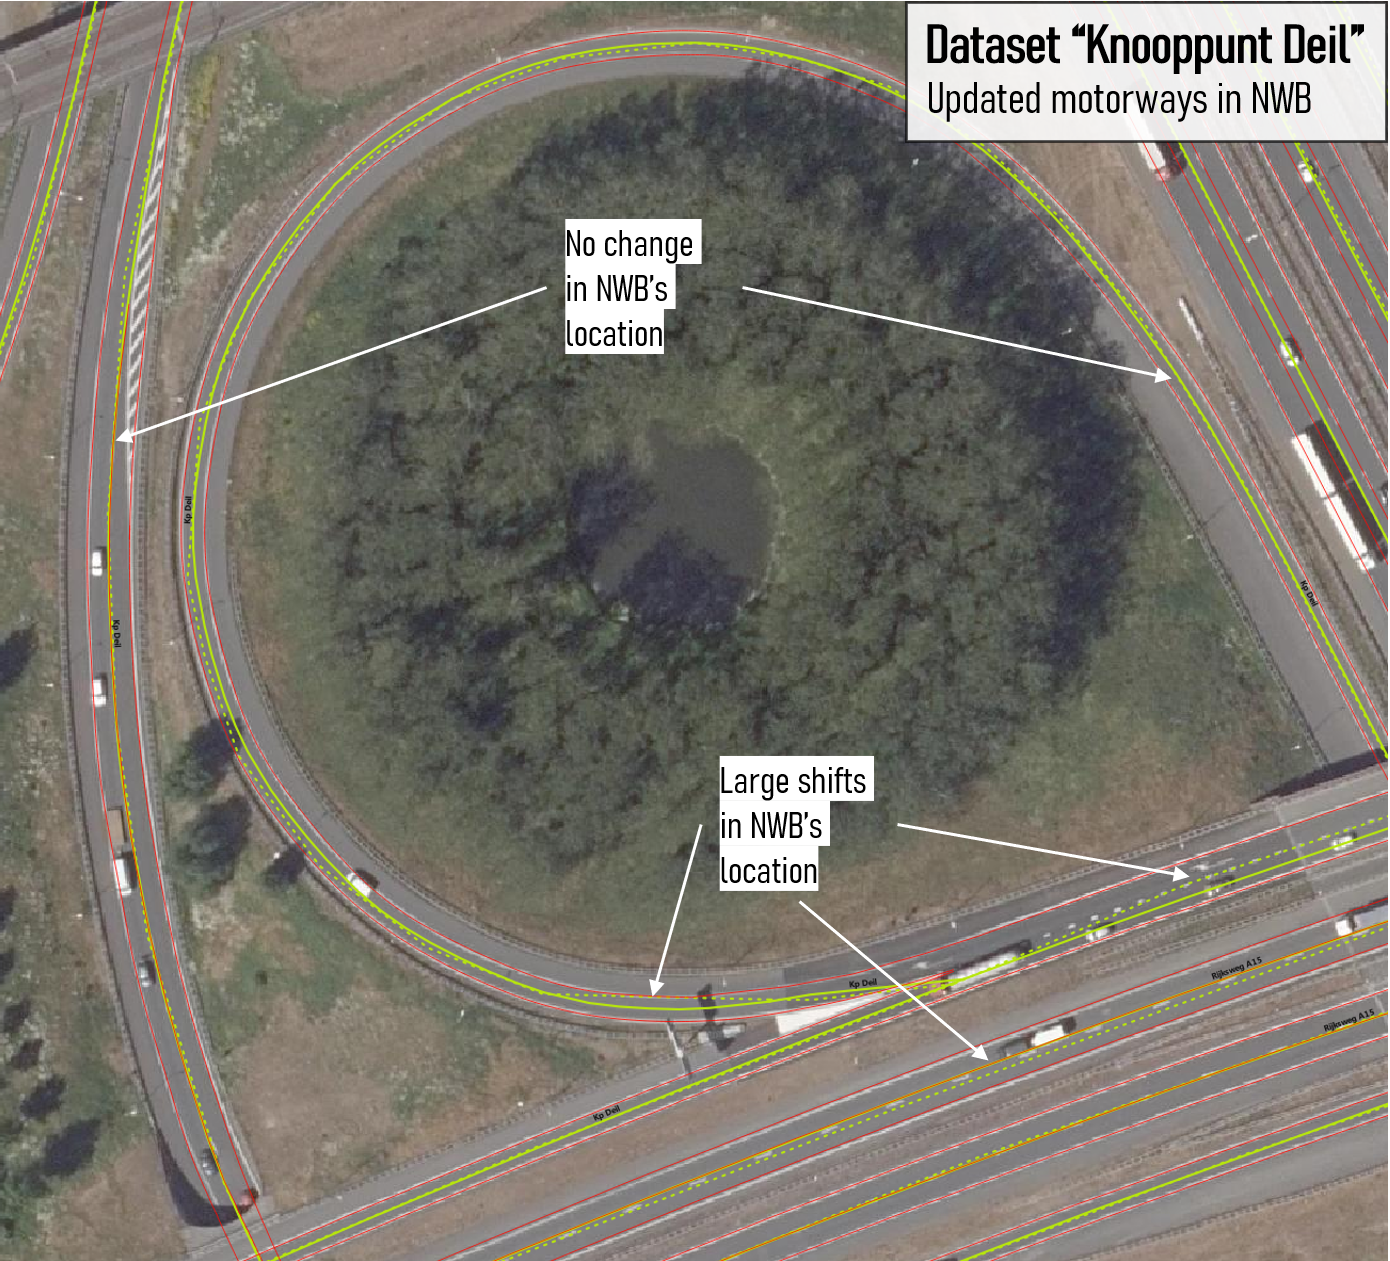
\includegraphics[width=0.84\linewidth]{final_report/figs/nwb_updated_geometry.png}
    \caption[Figure illustrating recent NWB improvements]{This 2D visualisation compares the original version of \ac{nwb} (on which the present research was based) to the newest release, in which \ac{r_road} centrelines were improved using \ac{dtb}. Solid green lines show the new position of the centrelines, while the dashed ones show the original ones. The thin red lines show the relevant \ac{dtb} features.}
    \label{fig:nwb_updated_geometry}
\end{figure}

\subsection{Impact on edge approximation}
\label{sub:nwb_updated_edgeapproximation}

The procedures from my processing pipeline that suffer the most from the \ac{nwb}-related issues are the edge approximation (and optimisation) and TIN construction workflows. In this section, I will discuss how edge approximation is affected by the improvements.

The main reason why edge approximation is sensitive to \ac{nwb}'s 2D location is that it assumes that the centrelines are always located on the road surfaces, and because the fixed-length cross-sections may extend into confusing areas if \ac{nwb} is close to either of the edges of a given road. For instance, if a centreline veers to the right and there is a flat region with a similar elevation beyond the edge of the road, the cross-section's elevations may not be classed as outliers there, in turn attracting the generated edges off the road. The workarounds I implemented to bypass the issue do not have a 100\% effectiveness, meaning that improvements to the 2D georeferencing accuracy of \ac{nwb} are expected to result in noticeable improvements in the effectiveness of this pipeline step.

Figure \ref{fig:nwb_updated_edgeapproximation} compares the generated edges prior to the refinement of the centrelines, and after. The main type of improvement noticeable in the new edges and cross-sections is that in bends, less cross-sections are skipped, and the new edges better define the extents of the road surfaces. The edges no longer contain short-wavelength extensions into off-road areas and are thus at a relatively constant distance from each other, even where the bends are quite sharp. This improvement is also noticeable where the same issue exists for the opposite reason (i.e. where \ac{nwb} is vastly oversimplified due to it being straight for a long distance).

The second, less intuitive improvement is due to the fact that already during the Lidar segmentation step, points relevant to the given road surface are selected more efficiently. Less off-road points being included in the queries results in the plane fits being more accurate. This bump in efficiency means that the algorithm now performs well in areas where it had failed before. In the upper visualisation in Figure \ref{fig:nwb_updated_edgeapproximation}, one of the \ac{nbrs} has been split in two due to the Lidar segmentation algorithm's inability to work properly around the entraces of the small tunnel that exists there. This also resulted in the \ac{dtb} points inside the tunnel not being found, which is why the \ac{nbrs} was split into two parts there.

With the new \ac{nwb} geometry, this is no longer an issue. Due to the improved georeferencing, the Lidar segmentation algorithm's plane fits are mostly defined by road surface points around the tunnel entrances, improving its performance drastically. The \ac{dtb} elevation measurements are found and used to navigate through the tunnel. Ultimately, the \ac{nbrs} needs not be split into two parts and several additional, meaningful cross-sections appear around the tunnel entrances, increasing the area properly covered by the generated road edges.

The improved edges also positively affect the performance of active contour optimisation, although not to an extent where re-introducing it into the recommended pipeline configuration would be justified.

\begin{figure}
    \centering
    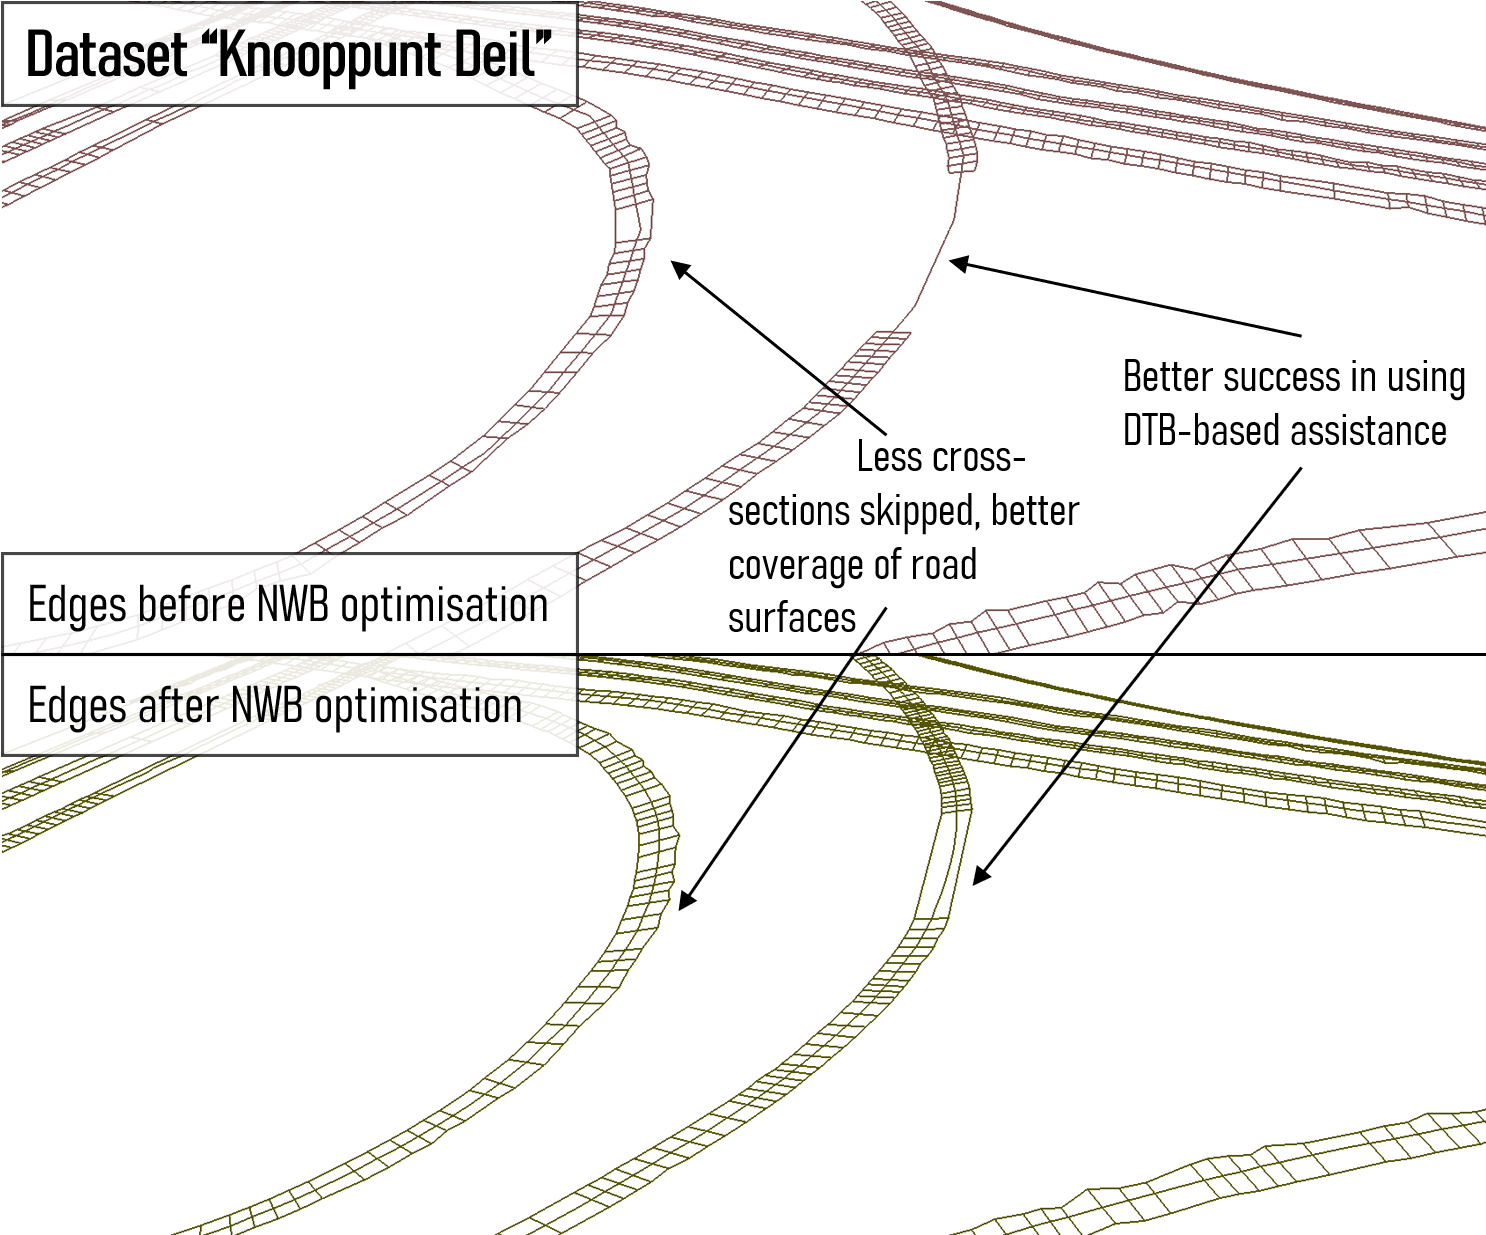
\includegraphics[width=0.8\linewidth]{final_report/figs/nwb_updated_edgeapproximation.png}
    \caption[Visualisation of the effects of improving NWB on preliminary edges]{This visualisation compares the cross-sections and preliminary edges generated using the original \ac{nwb} centrelines (above, in dark red) with the ones derived from the refined centrelines (below, in beige).}
    \label{fig:nwb_updated_edgeapproximation}
\end{figure}

\subsection{Impact on TIN construction}
\label{sub:nwb_updated_tinconstruction}

The \ac{tin} construction effectiveness also improves as a result of using corrected \ac{nwb} geometry. Figure \ref{fig:nwb_updated_tinconstruction} compares some of the \ac{tin}s before and after the refinement of \ac{nwb} in the same area as the one shown in Figures \ref{fig:nwb_updated_geometry} and \ref{fig:nwb_updated_edgeapproximation}. There are less off-road points between the updated edges (relative to the originals), and they better define the true road edges in general. This means that the seed line derived from them will also be more accurate.

As a result, the \ac{tin} initialisation step will be more reliable both in the seeding stage and during the conditional insertions that follow. Less off-road Lidar points will be tested with the (less strict) initialisation thresholds than before, since most of them will no longer fall between the road edges. Instead, they will be examined with the stricter insertion thresholds of the \ac{tin} extension stage. At the same time, many road surface points that were previously missing will now correctly lie between the road edges. This is likely to occur on the opposite side of the road relative to the side where off-road points were moved outside the edges. In simpler terms, moving the centreline in a certain direction often moves the preliminary edges in the same direction, which results in these two changes taking place simultaneously. It may also happen that one of the edges is left virtually unchanged while the other moves into its proper position, although this is somewhat rarer.

The fact that the edges extend closer towards areas with partial or full occlusion (such as the tunnel in this area) also means that the \ac{tin}s now also provide far better coverage in such regions. In fact, the \ac{tin} in this case extends all through the tunnel although this is not shown in the visualisation since the large tunnel-based triangles were removed when the \ac{tin}s were exported.

The latter improvement also benefits the generation of the final 3D-NWB geometries, since less elevations will need to be interpolated linearly. The former improvements (away from occluded areas) only have this effect where \ac{nwb}'s 2D referencing was so bad, that the preliminary edge approximation algorithm needed to skip enough cross-sections for the centreline to become located outside of the area delineated by the preliminary edges. This is extremely rare, hence we may safely conclude that the 3D-NWB elevations improve primarily in and directly around occluded lengths of roads.

\begin{figure}
    \centering
    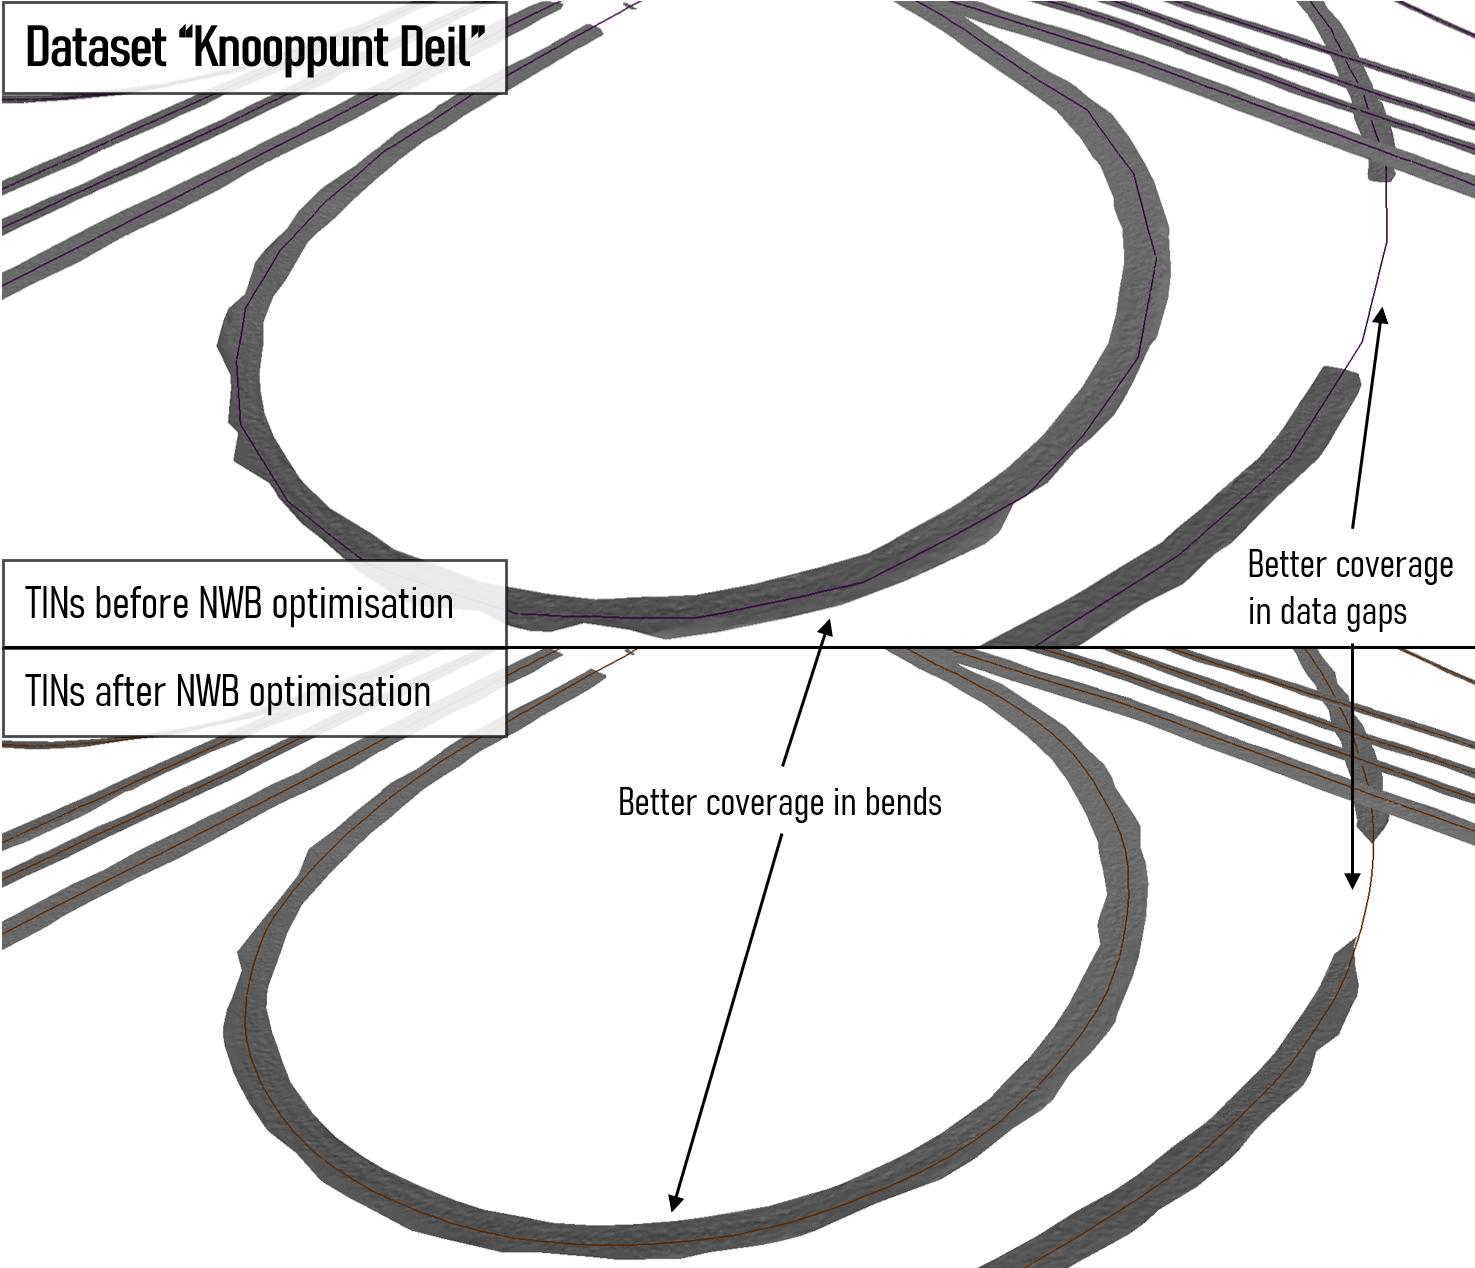
\includegraphics[width=0.8\linewidth]{final_report/figs/nwb_updated_tinconstruction.png}
    \caption[Visualisation of the effects of improving NWB on the TINs]{This visualisation compares the \ac{tin}s generated using the original \ac{nwb} centrelines (above) with the ones derived from the refined centrelines (below).}
    \label{fig:nwb_updated_tinconstructionn}
\end{figure}

\subsection{On improving NWB's 2D georeferencing dynamically}
\label{sub:nwb_updated_dynamic}

As the discussion and figures presented in this section indicate, improving \ac{nwb}'s stock georeferencing is certainly desirable, and \ac{ndw}'s recent efforts to realise this are already very promising. However, there are still many centrelines in \ac{nwb} which have not been refined yet, and even in the case of motorways, the refinement is only partial (because \ac{dtb} is incomplete).

My pipeline produces two main types of data: road surface \ac{tin} models and 3D-NWB geometry. Both of these appear to benefit significantly from improving the quality of the 2D georeferencing of the centrelines. However, some of these improvements may be possible to achieve internally, without relying on refinements carried out on \ac{nwb}. In other words, the georeferencing of \ac{nwb} could be improved dynamically at various points in my pipeline.

\subsubsection{Refinement during edge approximation}

In the \ac{tin} construction step, the \ac{tin}s are seeded via a seed line derived from the preliminary or optimised edges. Since the road edges are generated in a way that attempts to counteract the effects of \ac{nwb}'s coarse georeferencing, the seed line is often a more accurate representation of the road's centreline than \ac{nwb} is, itself. The same type of geometry could be easily derived already during the edge approximation step and then used as surrogate centrelines. It may be advisable to simplify or smooth the line somewhat, so that small-scale issues with the preliminary edges are not reflected in it. Before continuing, it would be necessary to perform edge approximation once again, but this time starting from the surrogate centreline. Without this additional step, the \ac{tin} construction stage would still make use of the \textit{original} preliminary edges, and not the ones that were improved based on the surrogate centrelines.

\subsubsection{Refinement during TIN construction}

Alternatively, one may instead attempt to derive the skeleton of the generated \ac{tin}s rather than that of the polygon formed by the preliminary or optimised edges. The edges of the road surface would first need to be located inside the generated \ac{tin}s. One could employ the same tactics that I utilised to export and visualise the models in this project, i.e. to remove large triangles and sliver triangles. The triangle edges that define the road edge could either be identified procedurally as part of the triangle removal step, or an $\alpha$-shape generation program could be used on the vertices of the accepted triangles.

To improve the \ac{tin}s based on the derived surrogate centrelines, the preliminary edges would then need to be re-generated and the \ac{tin}s would need to also be built from scratch again, based on the new edges. This would increase runtimes by a significant margin, hence performing centreline refinement as part of or as an extension of the edge approximation step is my recommendation.

\subsubsection{Effects on 3D-NWB}

The above refinements would primarily target the improvement of the generated \ac{tin}s via improving the centrelines. The surrogate centrelines would certainly not be accurate enough to be used in place of the original \ac{nwb} geometries when producing the output 3D-NWB geometries. Hence, the output centrelines would still be in the same horizontal locations as the original ones. However, since the \ac{tin}s would be more accurate, the elevation interpolation step would need to resort to linear interpolation less frequently. The improved \ac{tin}s, themselves, would be the other main reason why one may wish to add such routines to the pipeline.

I judge such methods not to be reliable enough to serve as a means to refine stock \ac{nwb} 2D georeferencing. Approaches that involve pre-existing \ac{rws} and third-party datasets (or surveying new data) are almost certainly better suited to this task, such as the approaches of the ongoing projects of \ac{ndw}.